\svnid{$Id: section_dockableviews.tex 1 2015-08-30 15:39:28Z mooiman $}

\section{Dockable views}
\label{sec:dockableviews}
The  framework offers lots of freedom to customize dockable views, which are discussed in this section.
\subsection{Docking tabs separately}
\label{subsec:dockingtabs}
Within the  framework the user can dock the separate windows according to personal preferences. These preferences are then saved for future use of the framework. An example of such preferences is presented in \Fref{fig:exampledocking}, where windows have been docked on two screens.
%
\begin{figure} [H]
	\centering
		\includegraphics[width=\textwidth]{Figures/Chapter_overview/example_docking.png}
	\caption{Docking windows on two screens within the framework.}
	\label{fig:exampledocking}
\end{figure}

\subsection{Multiple tabs}
\label{subsec:multipletabs}
In case two windows are docked in one view, the underlying window (tab) can be brought to the front by simply selecting the tab, as is shown here.
%
\begin{figure} [H]
	\centering
		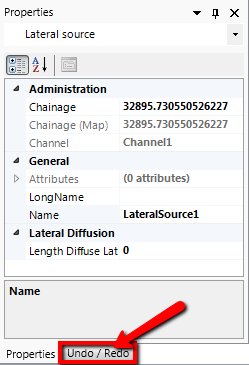
\includegraphics[width=0.5\textwidth]{Figures/Chapter_overview/example_docking_UndoRedo_1.png}
	\caption{Bringing the \window{Undo/Redo} window to the front}
\end{figure}
%
By dragging dockable windows with the left mouse button and dropping the window left, right, above or below another one the graphical user interface can be customized according to personal preferences. Here an example of the \window{Undo/Redo} window being docked above the \window{Properties} window.
%
\begin{figure} [H]
	\centering
		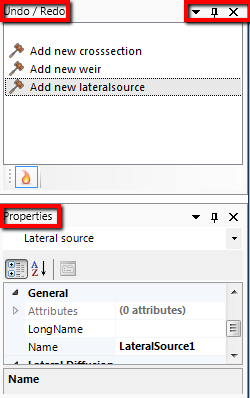
\includegraphics[width=0.5\textwidth]{Figures/Chapter_overview/example_docking_UndoRedo_2.png}
	\caption{Docking the \window{Undo/Redo} window.}
	\label{fig:docking}
\end{figure}
%
Additional features are the possibility to remove or (auto) hide the window (top right in \Fref{fig:docking}). In case of removal, the window can be retrieved by a mouse-click on \button{Undo/Redo} in the \menu{View} ribbon. Hiding the \window{Undo/Redo} window results in:
%
\begin{figure} [H]
	\centering
		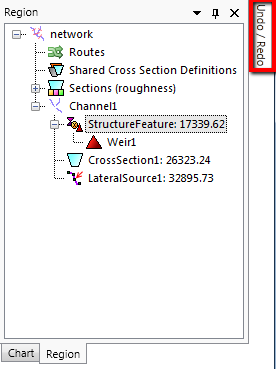
\includegraphics[width=0.5\textwidth]{Figures/Chapter_overview/example_autohide.png}
	\caption{Auto hide the \window{Undo / Redo} window}
\end{figure}